%% LyX 2.3.6.1 created this file.  For more info, see http://www.lyx.org/.
%% Do not edit unless you really know what you are doing.
\documentclass[english]{article}
\usepackage[T1]{fontenc}
\usepackage[latin9]{inputenc}
\usepackage{geometry}
\geometry{verbose,tmargin=2.5cm,bmargin=2.5cm,lmargin=2.5cm,rmargin=2.5cm}
\usepackage{array}
\usepackage{textcomp}
\usepackage{multirow}
\usepackage{amsmath}
\usepackage{graphicx}

\makeatletter

%%%%%%%%%%%%%%%%%%%%%%%%%%%%%% LyX specific LaTeX commands.
%% Because html converters don't know tabularnewline
\providecommand{\tabularnewline}{\\}

\makeatother

\usepackage{babel}
\begin{document}
{[}SPLIT\_HERE{]}
\begin{enumerate}
\item \textbf{{[}NJC/PRELIM/9597/2019/P1/Q1{]} }

The text files \texttt{WEATHER-JUNE-2018.TXT} and \texttt{WEATHER-JUNE-2019.TXT}
contain weather information in Singapore for the month of June in
both 2018 and 2019. Each line in either file contains tab delimited
data corresponding to (from the leftmost to the rightmost): 
\noindent \begin{center}
\begin{tabular}{|l|}
\hline 
Date\tabularnewline
\hline 
Daily Rainfall Total (mm)\tabularnewline
\hline 
Highest 30-min Rainfall (mm)\tabularnewline
\hline 
Highest 60-min Rainfall (mm)\tabularnewline
\hline 
Highest 120-min Rainfall (mm) \tabularnewline
\hline 
Mean Temperature (�C)\tabularnewline
\hline 
Maximum Temperature (�C)\tabularnewline
\hline 
Minimum Temperature (�C)\tabularnewline
\hline 
Mean Wind Speed (km/h)\tabularnewline
\hline 
Max Wind Speed (km/h)\tabularnewline
\hline 
\end{tabular}
\par\end{center}

The Date values are in the format: d(d) Mmm -- e.g., 1 Jun, 10 Jun.
All the remaining data values are stored as either integers (no decimal
place) or floating-point values (one decimal place). 

\subsection*{Task 1.1 }

Write the program code to read and store the data in both files. You
should use appropriate data structures to store this data such that
each individual value may be easily referenced. The data from each
file must be stored in different instances. 

\subsection*{Evidence 1 }

The program code for \textbf{Task 1.1}.\hfill{} {[}2{]}

In order to make a very simplistic observation on the effect of global
warming over the past year, you have been tasked to calculate the
median over the daily mean temperatures for the month of June in both
2018 and 2019. 

\subsection*{Task 1.2 }

Write the program code for a function that will sort each of the two
sets of data retrieved in \textbf{Task 1.1}. You are to implement
the Bubble Sort algorithm to perform this sorting. The Bubble Sort
algorithm should be applied to sort the records based on\textbf{ Mean
Temperature}. 

\subsection*{Evidence 2 }

The program code for \textbf{Task 1.2}.\hfill{} {[}5{]}

\subsection*{Task 1.3 }

Write the program code that utilises the Bubble Sort function implemented
in \textbf{Task 1.2} to calculate the \textbf{median} of the Mean
Temperatures from June 2018 and June 2019. Your program code should
then output the difference between the two temperatures. 

Sample output: 

\texttt{Difference in Median Temperatures (June 2019 \textendash{}
June 2018): 1.5�C}

\subsection*{Evidence 3 }

The program code for \textbf{Task 1.3}. \hfill{}{[}3{]}

In order to better study daily weather conditions, you must now also
create a simple textbased user interface that will allow the user
to search and output all temperatures (from both June 2018 and June
2019) that are above a certain mean temperature. 

The records that have a higher mean temperature than the specified
temperature should be output such that the following values are displayed: 
\noindent \begin{center}
\begin{tabular}{|l|}
\hline 
Date\tabularnewline
\hline 
Daily Rainfall Total (mm)\tabularnewline
\hline 
Mean Temperature (�C)\tabularnewline
\hline 
Mean Wind Speed (km/h)\tabularnewline
\hline 
\end{tabular}
\par\end{center}

The user interface should repeatedly prompt the user for a temperature
(i.e., a float). 

Sample input message:

\texttt{Please input a mean temperature threshold (�C):} 

Appropriate exception handling should be performed on user input,
with an appropriate warning given whenever incorrect input is specified. 

Once the user has input a temperature, the program should then output
all the records (from both the June 2018 and June 2019 files) that
have mean temperatures that are higher than the one specified. 

Sample output: 

\texttt{YEAR DATE ~~RAIN TEMP WIND }

\texttt{2018 7 Jun ~0 ~~~30.3 11.5 }

\texttt{2018 11 Jun 0 ~~~30.2 13.7 }

\texttt{2018 6 Jun ~0 ~~~30.2 12.6 }

\texttt{2019 10 Jun 0 ~~~30 ~~12.2 }

\texttt{2019 11 Jun 0 ~~~29.9 11.9 }

\texttt{2018 12 Jun 0 ~~~29.9 9.4 }

\texttt{2018 10 Jun 0 ~~~29.9 12.2 }

\texttt{2018 4 Jun ~0.4 ~29.7 7.9 }

\texttt{2019 28 Jun 0 ~~ 29.6 14.4}

\texttt{2018 17 Jun 0.4 ~29.6 11.9 }

Note that this output should be sorted in descending order of (mean)
temperature, and in the case of ties, in descending order of date.

\subsection*{Task 1.4 }

Write the program code for a function that performs an augmented Binary
Search. This function should use the sorted data from Task 1.1 to
search for the record that is just greater than a specified temperature
(i.e., the record with the lowest temperature that is just greater
than the specified temperature). 

\subsection*{Evidence 4 }

he program code for \textbf{Task 1.4}. \hfill{}{[}6{]}

\subsection*{Task 1.5 }

Write the program code that uses the augmented Binary Search function
implemented in \textbf{Task 1.4} to implement the user interface specified
above. 

\subsection*{Evidence 5 }

The program code for \textbf{Task 1.5}. \hfill{}{[}4{]}

{[}SPLIT\_HERE{]}
\item \textbf{{[}NJC/PRELIM/9597/2019/P1/Q2{]} }

While hunting for lost treasure, Lara happened upon an ancient scroll
that contains the following text (with some missing text denoted by
the underlined sections). 

\noindent %
\noindent\begin{minipage}[t]{1\columnwidth}%
\texttt{FUNCTION insertionSort(L: ARRAY OF INTEGER) RETURNS ARRAY
OF INTEGER }

\texttt{\qquad{}RETURN insertSortOuter(\_\_\_\_\_\_\_\_\_\_\_\_\_\_\_) }

\texttt{ENDFUNCTION \bigskip{}
}

\texttt{FUNCTION insertSortOuter(L: ARRAY OF INTEGER, i: INTEGER)
RETURNS ARRAY OF INTEGER }

\texttt{\qquad{}IF \_\_\_\_\_\_\_\_\_\_\_\_\_\_\_ THEN }

\texttt{\qquad{}\qquad{}RETURN L }

\texttt{\qquad{}ELSE}

\texttt{\qquad{}\qquad{}RETURN \_\_\_\_\_\_\_\_\_\_\_\_\_\_\_\_\_\_\_\_\_\_\_\_\_\_\_\_\_\_\_\_\_\_\_\_\_\_\_\_\_\_\_\_\_ }

\texttt{\qquad{}ENDIF }

\texttt{ENDFUNCTION \bigskip{}
}

\texttt{FUNCTION insertSortInner(L: ARRAY OF INTEGER, j: INTEGER)
RETURNS ARRAY OF INTEGER }

\texttt{\qquad{}IF \_\_\_\_\_\_\_\_\_\_\_\_\_\_\_ THEN }

\texttt{\qquad{}\qquad{}RETURN L}

\texttt{\qquad{}ELSE }

\texttt{\qquad{}\qquad{}IF \_\_\_\_\_\_\_\_\_\_\_\_\_\_\_ THEN \_\_\_\_\_\_\_\_\_\_\_\_\_\_\_\_\_\_\_\_\_}

\texttt{\qquad{}\qquad{}\qquad{}\_\_\_\_\_\_\_\_\_\_\_\_\_\_\_\_\_\_\_\_\_\_\_\_ }

\texttt{\qquad{}\qquad{}ENDIF }

\texttt{\qquad{}\qquad{}RETURN \_\_\_\_\_\_\_\_\_\_\_\_\_\_\_\_\_\_\_\_\_\_\_\_\_\_\_\_\_\_ }

\texttt{\qquad{}ENDIF }

\texttt{ENDFUNCTION }%
\end{minipage}

Assist Lara by completing the above code. 

\subsection*{Task 2.1 }

Write the program code for a recursive implementation of the Insertion
Sort algorithm (based on the functions defined above). 

\subsection*{Evidence 6 }

The program code for Task 2.1.\hfill{} {[}6{]}

Lara is not completely sure that your implementation really works
and asks you to provide proof that it works correctly. 

\subsection*{Task 2.2 }

Design a set of test cases to test the algorithm you implemented in
\textbf{Task 2.1}. 

\subsection*{Evidence 7}

The table of test cases to test the program code implemented in \textbf{Task
2.1}. \hfill{}{[}2{]}

On another adventure, Lara happens upon a puzzle that requires the
calculation of Fibonacci Numbers. 

Once again, she enlists your help, and tasks you to assist her with
the computation of these numbers. However, since she abhors loops,
your implementation must be fully recursive (and thus, not include
the use of any loops -- i.e., no \texttt{while} or \texttt{for} statements). 

Note that the Fibonacci Number sequence, $F_{0}$, $F_{1}$, $F_{2}$,
\dots , is defined as follows: 
\begin{align*}
F_{0} & =0\\
F_{1} & =1\\
 & \vdots\\
F_{i} & =F_{i-1}+F_{i-2}
\end{align*}

More specifically, you are required to write a function that: 
\begin{itemize}
\item Takes one positive integer value as input, $n$
\item If $n$ is a Fibonacci Number, then determine (recursively), the smallest
integer k, where $n=F_{k}$, the $k$-th Fibonacci Number, and return
the value $k$ 
\item Or else, if $n$ is not a Fibonacci Number, return the value -1 
\end{itemize}

\subsection*{Task 2.3 }

Write the program code for a recursive function, where no loops are
used, to implement the algorithm described above. 

\subsection*{Evidence 8 }

The program code for Task 2.3. \hfill{}{[}8{]}

\subsection*{Task 2.4}

Design a set of test cases to test the algorithm you implemented in
Task 2.3. 

\subsection*{Evidence 9 }

The table of test cases to test the program code implemented in Task
2.3.\hfill{} {[}2{]}

\subsection*{Task 2.5}

Write the program code (using your implementation of the algorithm
in Task 2.3) to determine if the output for the integers: 1346270
and 24157817. 

\subsection*{Evidence 10 }

The program code to test the implementation in Task 2.3 (using cases
in Task 2.4). \hfill{}{[}2{]}

{[}SPLIT\_HERE{]}
\item \textbf{{[}NJC/PRELIM/9597/2019/P1/Q3{]} }

Desmond wishes to implement a Hybrid Data Structure (HDS) using object-oriented
programming (OOP). This HDS is meant to store telephone numbers in
the following format (as a string). 
\noindent \begin{center}
<Country Code String><Space Character><Number in Country String> 
\par\end{center}

The Country Code String may include: 
\begin{itemize}
\item Any digit -- i.e., 0 to 9 
\item A dash -- i.e., \textquotedblleft -\textquotedblright{} 
\end{itemize}
The Number in Country String may only include digits. It also includes
any city codes, etc. 

Consequently, you are to implement the following \texttt{PhoneNum}
class.
\noindent \begin{center}
\begin{tabular}{|c|}
\hline 
\texttt{STRING}\tabularnewline
\hline 
\tabularnewline
\hline 
\tabularnewline
\hline 
\multicolumn{1}{c}{\texttt{$\uparrow$}}\tabularnewline
\hline 
\texttt{PhoneNum}\tabularnewline
\hline 
\tabularnewline
\hline 
\texttt{+hash() : INTEGER}\tabularnewline
\hline 
\end{tabular}
\par\end{center}

\begin{tabular*}{0.1\paperwidth}{@{\extracolsep{\fill}}|c|c|}
\hline 
\textbf{Attribute/Method} & \textbf{Description}\tabularnewline
\hline 
\texttt{PhoneNum.hash()} & This overwrites the default hash method and is calculated based on:
((ASCII value of char at index i) {*} i), for each element i in the
word stored. Note that the value of i is based on 1-indexed indexing.\tabularnewline
\hline 
\end{tabular*}

\subsection*{Task 3.1 }

Write the program code to implement the \texttt{PhoneNum} class. 

\subsection*{Evidence 11 }

The program code for \textbf{Task 3.1}. \hfill{} {[}3{]}

The HDS specifically corresponds to a Linked List (LL), where each
node in this LL is also the root of a Binary Search Tree (BST). 
\begin{center}
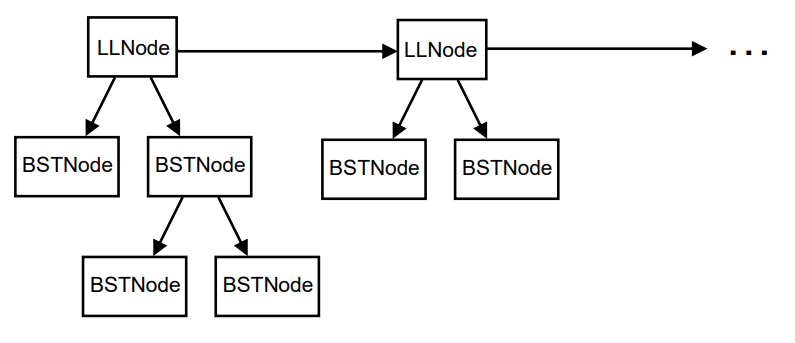
\includegraphics[width=0.5\paperwidth]{C:/Users/Admin/Desktop/Github/question_bank/LyX/static/img/9597-NJC-2017-P1-Q3-1}
\par\end{center}

Essentially, each LLNode stores a telephone number from a unique country,
as defined by the <Country Code String> part of the string within
each \texttt{PhoneNum} instance. Thus, among all the \texttt{PhoneNum}
instances stored in LLNodes, there cannot be any instances that share
the same Country Code String. 

The BSTNodes are sorted based on the Hash Value of each \texttt{PhoneNum}
instance. 

It should also be noted that all \texttt{PhoneNum} instances are to
be stored within an array in the HDS, and as such, all links stored
in nodes are integers corresponding to indices within this array. 

Consequently, you are to implement the following classes for the HDS. 
\noindent \begin{center}
\begin{tabular}{|l|}
\hline 
\texttt{Node}\tabularnewline
\hline 
\texttt{-data : PhoneNum}\tabularnewline
\texttt{-link1: INTEGER}\tabularnewline
\texttt{-link2: INTEGER}\tabularnewline
\texttt{-link3: INTEGER}\tabularnewline
\hline 
\texttt{+constructor()}\tabularnewline
\texttt{+getData() : STRING}\tabularnewline
\texttt{+setData(STRING)}\tabularnewline
\texttt{+getLink1() : INTEGER}\tabularnewline
\texttt{+setLink1(INTEGER)}\tabularnewline
\texttt{+getLink2() : INTEGER}\tabularnewline
\texttt{+setLink2(INTEGER)}\tabularnewline
\texttt{+getLink3() : INTEGER}\tabularnewline
\texttt{+setLink3(INTEGER)}\tabularnewline
\texttt{+print()}\tabularnewline
\hline 
\end{tabular}%
\begin{tabular}{|l|}
\hline 
\texttt{HDS}\tabularnewline
\hline 
\texttt{-nodes : ARRAY OF NODES}\tabularnewline
\texttt{-free: INTEGER}\tabularnewline
\texttt{-first: INTEGER}\tabularnewline
\hline 
\texttt{+constructor(INTEGER)}\tabularnewline
\texttt{+insert(PhoneNum)}\tabularnewline
\texttt{+contains(PhoneNum)}\tabularnewline
\texttt{+print()}\tabularnewline
\hline 
\end{tabular}
\par\end{center}

Since each LLNode is also the root node of its corresponding BST,
the \texttt{Node} class defined above is used to represent both LLNodes
and BSTNodes. 

The \texttt{link2} and \texttt{link3} attributes always correspond
to the left and right nodes of the BST, whereas \texttt{link1} corresponds
to either: (a) the next link in the LL when the node in question is
a LLNode; or (b) the previous link in the BST when the node in question
is a BSTNode. BSTNode BSTNode BSTNode BSTNode BSTNode BSTNode LLNode
LLNode \dots{} 8 NJC Mathematics 2019 9597/01/O/N/19

The following are the descriptions of the various attributes and methods
within the abovementioned Node and HDS classes. 

\begin{tabular*}{0.1\paperwidth}{@{\extracolsep{\fill}}|l|l|}
\hline 
\textbf{Attribute/Method} & \textbf{Description}\tabularnewline
\hline 
\texttt{Node.constructor()} & Initialisation of a \texttt{Node} instance assigns the value\texttt{
-1} to \texttt{link1}, \texttt{link2}, and \texttt{link3} attributes,
and a \texttt{NULL} value to the \texttt{data} attribute.\tabularnewline
\hline 
\texttt{Node.data} & This attribute is used to store an instance of \texttt{PhoneNum}.\tabularnewline
\hline 
\texttt{Node.link1 } & \multirow{3}{*}{Each of these attributes references an index (i.e., integer) from
\texttt{HDS.nodes}. To indicate an empty reference, the value\texttt{
-1} is used. When the \texttt{Node} instance in question corresponds
to a LLNode, \texttt{link1} corresponds to the index of the next LLNode.
When the Node instance in question corresponds to a BSTNode, \texttt{link1}
corresponds to the index of the previous BSTNode (of LLNode). The
\texttt{link2} and \texttt{link3} attributes always correspond to
the indices of the left and right nodes in the BST.}\tabularnewline
\texttt{Node.link2} & \tabularnewline
\texttt{Node.link3} & \tabularnewline
\hline 
\texttt{Node.print()} & This method should output the integer values stored in \texttt{link1},
\texttt{link2}, and \texttt{link3}, as well as the value in data the
following format: \texttt{DATA: <STRING>; HASH: <INTEGER>; LINK1: <INTEGER>;
LINK2: <INTEGER>; LINK3: <INTEGER>}\tabularnewline
\hline 
\texttt{HDS.nodes } & \multirow{3}{*}{The attribute \texttt{HDS.nodes} corresponds to an array of 25 \texttt{Node}
instances. This array is to be pre-initialised with 25 unused \texttt{Node}
instances. This value should be specified on creation of the new instance
(i.e., as an argument). The \texttt{HDS.free} attribute references
the index of the head (i.e., first node) of a singly-linked linked
list of empty \texttt{Node} instances. The \texttt{Node.link1} values
are used to reference each subsequent node index in this linked list.
When initialising the \texttt{HDS.nodes} attribute, you must ensure
that this linked list of free nodes is initialised as well. The \texttt{HDS.first}
attribute references index of the head (i.e., first node) of the actual
HDS.}\tabularnewline
\texttt{HDS.free } & \tabularnewline
\texttt{HDS.first} & \tabularnewline
\hline 
\texttt{HDS.insert(PhoneNum)} & The \texttt{HDS.insert} method takes a \texttt{PhoneNum} instance
as input and inserts it into the HDS. Note that each \texttt{Node}
instance inserted into the actual HDS must correspond to a \texttt{Node}
instance from the LL of free nodes, which is referenced by the head
of the free node LL at the index stored in the attribute \texttt{HDS.free}.
Insertion requires you to first remove the node from the LL of free
nodes before inserting it into the actual HDS. When inserting into
the HDS, you must first check the Country Code String part of \texttt{PhoneNum}
and insert it into the LL part of the HDS only if that country code
does not already exist in the LL part of HDS. If the Country Code
String part of the \texttt{PhoneNum} instance in question does exist
(in the LL part of the HDS), then it is instead to be inserted into
the BST whose root shares the same Country Code String. When inserting
into a BST within the HDS, do recall that within each BST, nodes are
sorted based on Hash Value.\tabularnewline
\hline 
\texttt{HDS.contains(PhoneNum)} & This method will return True if the given \texttt{PhoneNum} instance
exists within the \texttt{HDS}, or else returns False.\tabularnewline
\hline 
\texttt{HDS.print()} & Prints the contents of \texttt{HDS.nodes} in index order. Note that
to print each \texttt{Node} instance within \texttt{HDS.nodes}, \texttt{Node.print()}
should be called.\tabularnewline
\hline 
\end{tabular*}

\subsection*{Task 3.2 }

Write the program code to implement the \texttt{Node} class.

\subsection*{Evidence 12 }

The program code for \textbf{Task 3.2}. \hfill{} {[}4{]}

\subsection*{Task 3.3 }

Write the program code to implement the \texttt{HDS} class, excluding
the \texttt{insert} and \texttt{contains} methods. 

\subsection*{Evidence 13 }

The program code for \textbf{Task 3.3}. \hfill{}{[}5{]}

\subsection*{Task 3.4 }

Write the program code to implement the \texttt{insert} method for
the \texttt{HDS} class. 

\subsection*{Evidence 14 }

The program code for \textbf{Task 3.4}. \hfill{}{[}13{]}

\subsection*{Task 3.5 }

Write the program code to implement the \texttt{contains} method for
the \texttt{HDS} class. 

\subsection*{Evidence 15 }

The program code for \textbf{Task 3.5}. \hfill{} {[}7{]}

\subsection*{Task 3.6 }

Write the program code to initialise a \texttt{HDS} and store the
contents of \texttt{PHONENUMS.TXT}. as \texttt{PhoneNum} instances
within the initialised \texttt{HDS}. Then print the contents of the
HDS. 

\subsection*{Evidence 16 }

The program code for \textbf{Task 3.6}. \hfill{}{[}3{]}

\subsection*{Evidence 17 }

The screenshot output corresponding to\textbf{ Task 3.6}. \hfill{}{[}1{]}

\subsection*{Task 3.7 }

Write the program code for the \texttt{HDS.orderedPrint} method, which
uses in-order traversal on each BST within the HDS. 

\subsection*{Evidence 18 }

The program code for \textbf{Task 3.7}. \hfill{}{[}4{]}

{[}SPLIT\_HERE{]}
\item \textbf{{[}NJC/PRELIM/9597/2019/P1/Q4{]} }

The Hex game involves an $n\times n$ hexagonal board. An example
of a $3\times3$ Hex board is thus as follows. 
\begin{center}
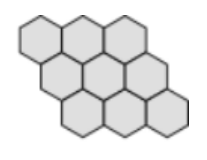
\includegraphics[width=0.15\paperwidth]{C:/Users/Admin/Desktop/Github/question_bank/LyX/static/img/9597-NJC-2019-P1-Q4-1}
\par\end{center}

Hex is a two-player game, where one player must build a bridge that
extends from left to right, and the other player must build a bridge
that extends from top to bottom. 

Each player takes turns to play, and may place a piece in any empty
cell. 

The following is an example board where the X player (going from left
to right) has won the game. 
\begin{center}
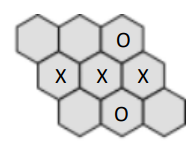
\includegraphics[width=0.15\paperwidth]{C:/Users/Admin/Desktop/Github/question_bank/LyX/static/img/9597-NJC-2019-P1-Q4-2}
\par\end{center}

The following is an example board where the O player (going from top
to bottom) has won the game. 
\begin{center}
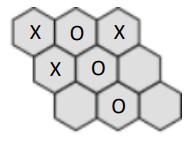
\includegraphics[width=0.15\paperwidth]{C:/Users/Admin/Desktop/Github/question_bank/LyX/static/img/9597-NJC-2019-P1-Q4-3}
\par\end{center}

The representation for a Hex Board may be based on a standard 2-dimensional
Array. Essentially, the Hex Board may be referenced as a 2-dimensional
Array as follows. 
\begin{center}
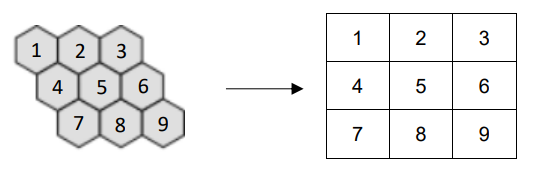
\includegraphics[width=0.5\paperwidth]{C:/Users/Admin/Desktop/Github/question_bank/LyX/static/img/9597-NJC-2019-P1-Q4-4}
\par\end{center}

You are tasked to design an object oriented programming class to store
the Hex Board. This class, \texttt{HexBoard}, should be implemented
as follows.
\begin{center}
\begin{tabular}{|l|}
\hline 
\texttt{HexBoard}\tabularnewline
\hline 
\texttt{- board: ARRAY OF ARRAY OF STRING}\tabularnewline
\texttt{- turn: INTEGER }\tabularnewline
\hline 
\texttt{+constructor(INTEGER) }\tabularnewline
\texttt{+playX(INTEGER, INTEGER) }\tabularnewline
\texttt{+playO(INTEGER, INTEGER)}\tabularnewline
\texttt{+checkWinX(): BOOLEAN}\tabularnewline
\texttt{+checkWinO(): BOOLEAN}\tabularnewline
\texttt{+printBoard()}\tabularnewline
\hline 
\end{tabular}
\par\end{center}

\begin{tabular*}{0.1\paperwidth}{@{\extracolsep{\fill}}|l|l|}
\hline 
\textbf{Attribute/Method} & \textbf{Description}\tabularnewline
\hline 
\texttt{HexBoard.constructor (INTEGER) } & Initialises the \texttt{board} attribute as a 2D Array of Strings.
The size of each array (both outer and inner arrays) are based on
the specified integer value. The \texttt{turn} attribute is initialised
as 0.\tabularnewline
\hline 
\texttt{HexBoard.playX (INTEGER, INTEGER)} & This method allows the X player to make a move by specifying the coordinates
where he or she wished to place an X piece.\tabularnewline
\hline 
\multirow{3}{*}{\texttt{HexBoard.playO (INTEGER, INTEGER)}} & \multirow{3}{*}{This method allows the O player to make a move by specifying the coordinates
where he or she wished to place an O piece.}\tabularnewline
 & \tabularnewline
 & \tabularnewline
\hline 
\texttt{HexBoard.checkWinX(): BOOLEAN} & This method checks the board and returns True if the X player has
won the game, or else returns False.\tabularnewline
\hline 
\multirow{3}{*}{\texttt{HexBoard.checkWinO(): BOOLEAN}} & \multirow{3}{*}{This method checks the board and returns True if the O player has
won the game, or else returns False. }\tabularnewline
 & \tabularnewline
 & \tabularnewline
\hline 
\texttt{HexBoard.printBoard()} & This method prints the contents of the board using the 2D Array representation. \tabularnewline
\hline 
\end{tabular*}

\subsection*{Task 4.1}

Write the program code to implement the \texttt{HexBoard} class, excluding
the \texttt{checkWinX} and \texttt{checkWinO} methods. Your solution
\textbf{must work for any board size}.

\subsection*{Evidence 19 }

The program code for \textbf{Task 4.1}. \hfill{}{[}4{]}

\subsection*{Task 4.2 }

Write the program code to implement the \texttt{checkWinX} and \texttt{checkWinO}
methods.

\subsection*{Evidence 20 }

The program code for\textbf{ Task 4.2}. \hfill{}{[}12{]}

\subsection*{Task 4.3 }

Write the program code to test the following 4 test cases for both
X and O. 
\begin{center}
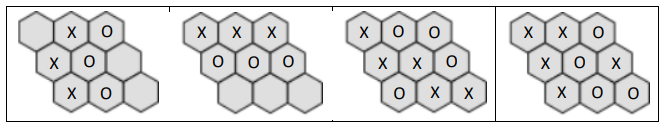
\includegraphics[width=0.5\paperwidth]{C:/Users/Admin/Desktop/Github/question_bank/LyX/static/img/9597-NJC-2019-P1-Q4-5}
\par\end{center}

Note that X wins by forming a bridge from left to right, while O wins
by forming a bridge from top to bottom. 

\subsection*{Evidence 21 }

The screenshots of the inputs and outputs to test each of the above
cases. \hfill{} {[}4{]}

{[}SPLIT\_HERE{]}
\item \textbf{{[}NJC/PRELIM/9597/2019/P2/Q1{]} }

At Central Secondary School, the current system for tracking Co-Curricular
Activity (CCA) equipment requires manual updating. More specifically,
the teachers in-charge of CCAs manage printed records of their equipment
inventories. 

In this system, stock-taking of equipment is performed once per year,
where teachers and students perform a physical count of each item
on an inventory list. At this point, any damaged or lost items are
flagged, and then replacements are ordered. To process orders, requests
are submitted to the general office. 

A new automated system that utilises Radio-frequency identification
(RFID) tags has been proposed. The proposal is to use passive RFID
tags, which, unlike a barcode, do not need to be within the line of
sight of the reader, so it may be embedded in the tracked object. 

Within the proposed system, each piece of CCA equipment will be embedded
with an RFID tag, which would allow them to be easily tracked. Tracking
is performed by several RFID readers that will be positioned at various
venues where CCA equipment are typically stored. Teacher and staff
may access this data by physically linking a computer to each RFID
reader. 

The main idea behind the proposed system is to have an inventory system
that may be continuously updated, which would remove the need for
the annual stock-taking exercise, and ensure that inventory is replenished
in a timelier fashion. 
\begin{enumerate}
\item Describe \textbf{two} feasibility study constraints that are relevant
to the above project. \hfill{}{[}2{]}
\item The proposed system is a complete overhaul of the exiting system.
What other alternative solutions are typically applicable to a system?
Suggest one example of each such solution that would be applicable
to the given context. \hfill{}{[}4{]}
\end{enumerate}
Once the feasibility study is concluded, the school moves ahead with
the project using the following schedule.
\noindent \begin{center}
\begin{tabular}{|c|l|c|c|c|c|}
\hline 
\multirow{2}{*}{\textbf{Activity}} & \multirow{2}{*}{\textbf{Description}} & \multirow{2}{*}{\textbf{Preceding Activity}} & \multicolumn{3}{c|}{\textbf{Duration (weeks)}}\tabularnewline
\cline{4-6} \cline{5-6} \cline{6-6} 
 &  &  & \textbf{Worst} & \textbf{Expected} & \textbf{Best}\tabularnewline
\hline 
A & Analysis of requirements & - & 4 & 2 & 1\tabularnewline
\hline 
B & Design of the system & A & 10 & 7 & 3\tabularnewline
\hline 
C & Writing system documentation & A & 24 & 18 & 12\tabularnewline
\hline 
D & Implementation of the system & B & 17 & 14 & 12\tabularnewline
\hline 
E & Unit Testing & B & 12 & 7 & 4\tabularnewline
\hline 
F & Integration Testing & E & 8 & 5 & 3\tabularnewline
\hline 
G & Installation of the system & D, F & 10 & 3 & 2\tabularnewline
\hline 
H & Evaluation of the system & C, G & 4 & 2 & 1\tabularnewline
\hline 
\end{tabular}
\par\end{center}
\begin{enumerate}
\item[(c)]  Describe \textbf{two} things that a systems analyst might do in
order to determine the requirements of the new system. \hfill{}{[}2{]}
\item[(d)]  Draw a Data Flow Diagram (DFD) to describe the existing (manual)
CCA equipment inventory system. \hfill{}{[}4{]}
\item[(e)]  During which phases of the SDLC are DFDs utilised? Also, name the
specific documentation that includes them. \hfill{}{[}4{]}
\item[(f)]  PERT charts utilise a weighted average. Determine the weighted average
for each of the activities listed. \hfill{}{[}1{]}
\item[(g)]  Draw the network PERT chart diagram for the above project schedule.
This PERT chart should clearly indicate the dummy activities within
the project. \hfill{} {[}3{]}
\item[(h)]  Draw the PERT chart for the above, completing both the forward and
backward pass in order to determine the slack time for each activity.
\hfill{} {[}3{]}
\item[(i)]  For a general Systems Development project, during which phase of
the SDLC are PERT and Gantt Charts typically generated? Explain why
they are not generated in other phases instead. \hfill{} {[}2{]}
\item[(j)]  During which phase is the test plan typically created? \hfill{}
{[}1{]}
\item[(k)]  When implementing the system, one of several SDLC methodologies
may be adopted. List \textbf{three} such methodologies. \hfill{}{[}3{]}
\item[(l)]  Among the methodologies you have listed in your answer to part \textbf{(j)}
above, pick one that is relevant to the give context. Justify your
answer by contrasting your answer against the methodology proposed
within the given context. \hfill{}{[}3{]}
\item[(m)]  User and support staff training is an important part of the SDLC.
Which phase includes such training? \hfill{} {[}1{]}
\item[(n)]  The maintenance phase, while not included in the given schedule,
is important to a project. Describe two forms of maintenance that
would be relevant to the proposed system. Justify each choice. \hfill{}
{[}2{]}
\end{enumerate}
The proposed network design for the RFID CCA Inventory system is as
follows: 

Each CCA Store room will have a set of RFID-Reader linked to a desktop
computer. The computers in every CCA Store need to be able to access
a centralised database server to update the inventory records. The
database server is physically located in another room in the same
building as all the CCA store rooms.
\begin{center}
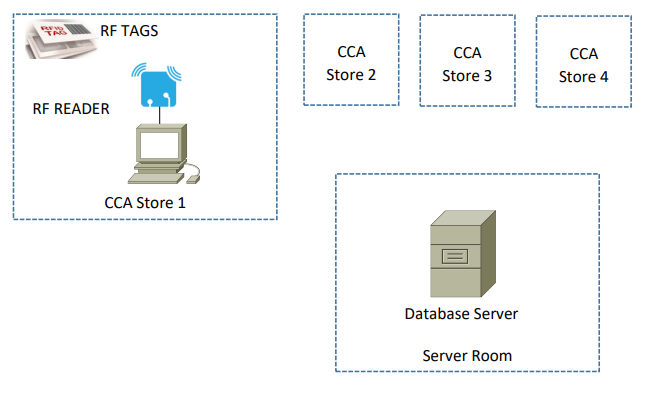
\includegraphics[width=0.5\paperwidth]{C:/Users/Admin/Desktop/Github/question_bank/LyX/static/img/9597-NJC-2019-P2-Q1-1}
\par\end{center}
\begin{enumerate}
\item[(o)]  Based on the diagram above, draw a network diagram to include the
physical/wireless connections and network equipment/s required to
implement the physical network. Label the equipment and connections
used in the diagram \hfill{} {[}2{]}
\item[(p)]  Describe the transmission mode used between RF Reader and the RF
TAGS in terms of how data is transferred between them. Justify your
answer. \hfill{}{[}1{]}
\end{enumerate}
After the proposed system has been implemented successfully, the school
is considering a Phase 2 implementation to include embedding RFID
tags to the school badges worn by the students and placing RFID readers
in different locations within the school compound. This will allow
attendance to be taken automatically and to track the movement of
students in the school. 

Given the fact that passive RFID tags do not have any access control
system, any commercially available RFID reader sold in the market,
is capable of accessing the information stored in the RFID tags. 
\begin{enumerate}
\item[(q)]  As a project manager for this project, you are to list and describe
two ethical implications in the proposed Phase 2 implementation. \hfill{}{[}2{]}
\end{enumerate}
{[}SPLIT\_HERE{]}
\item \textbf{{[}NJC/PRELIM/9597/2019/P2/Q2{]} }
\begin{enumerate}
\item Command line interfaces and graphical user interfaces are two common
forms of user interface. Explain the difference between the two, emphasising
when each is more applicable. \hfill{}{[}2{]}
\item There are typically eight qualities that good interfaces possess.
List and describe four. \hfill{} {[}4{]}
\end{enumerate}
\item \textbf{{[}NJC/PRELIM/9597/2019/P2/Q3{]} }

Pascal\textquoteright s Triangle follows the pattern below. 
\begin{center}
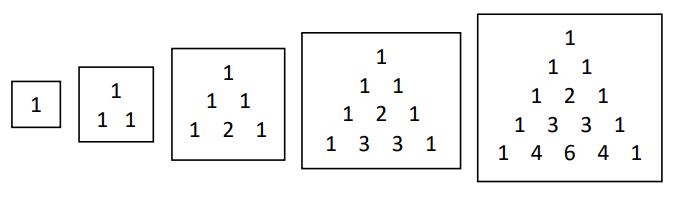
\includegraphics[width=0.5\paperwidth]{C:/Users/Admin/Desktop/Github/question_bank/LyX/static/img/9597-NJC-2019-P2-Q3-1}
\par\end{center}

These correspond to the Pascal\textquoteright s Triangles for $n=1$
(leftmost) to $n=5$ (rightmost). 
\begin{enumerate}
\item Write the Pseudocode for a function that will iteratively (i.e., not
recursively) print the Pascal\textquoteright s Triangle of depth $n$,
where $n$ is the only parameter of this function. You may not use
the binomial coefficient formula or use factorial calculations within
this implementation. 

Note that in your implementation, you need not worry about the centring
the triangle. For example, when $n=5$, you may instead output: 
\begin{center}
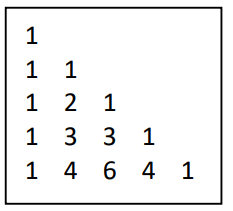
\includegraphics[width=0.15\paperwidth]{C:/Users/Admin/Desktop/Github/question_bank/LyX/static/img/9597-NJC-2019-P2-Q3-2}
\par\end{center}

\hfill{}{[}4{]}
\item Design a valid boundary test case for the function implemented in
\textbf{(a)}. \hfill{} {[}1{]}
\item Re-write your function such it is now fully recursive (i.e., does
not utilise any loops). \hfill{}{[}4{]}
\item Trace your recursive implementation for $n=3$. \hfill{}{[}3{]}
\end{enumerate}
{[}SPLIT\_HERE{]}
\item \textbf{{[}NJC/PRELIM/9597/2019/P2/Q4{]} }
\begin{enumerate}
\item Stacks and queues may be implemented using a Singly-linked Linked
List (LL) if we desire them to be dynamically sized. 
\begin{enumerate}
\item Using Object Oriented Programming (OOP), design a fully modular implementation
for a linked list and the corresponding stack and queue structures.
You need only specify the UML Class Diagrams for all the necessary
classes. All necessary attributes and methods must be listed, and
your solution must indicate any inheritance and polymorphism that
is necessary to achieve full modularity. \hfill{} {[}4{]}
\item Explain why a Singly-linked linked list is used, instead of a Doubly
or Doublycircular linked list. \hfill{}{[}1{]}
\end{enumerate}
\item When implementing a Hash Table, it is typically necessary to ensure
that your implementation also includes collision resolution. Two categories
of collision resolution mechanisms for Hash Tables are Open Addressing
and Separate Chaining. 
\begin{enumerate}
\item Describe the algorithm for the opening addressing mechanism of quadratic
probing. \hfill{}{[}3{]}
\item Describe the difference between linear probing and quadratic probing,
and explain why one might wish to use quadratic probing instead of
linear probing. \hfill{}{[}2{]}
\end{enumerate}
A computer scientist has implemented the following \texttt{INSERT}
function for a Hash Table. 

\noindent %
\noindent\begin{minipage}[t]{1\columnwidth}%
\texttt{FUNCTION INSERT(hashTable: ARRAY OF OBJECT, data: OBJECT) }

\texttt{RETURNS ARRAY OF OBJECT }

\texttt{\qquad{}DECLARE hashValue, step: INTEGER }

\texttt{\qquad{}IF ISFULL(hashTable) THEN }

\texttt{\qquad{}\qquad{}OUTPUT \textquotedbl Hash Table full. Unable
to insert.\textquotedbl}

\texttt{\qquad{}\qquad{}RETURN NULL }

\texttt{\qquad{}ENDIF }

\texttt{\qquad{}hashValue <- HASH(data) \% hashTable.SIZE() }

\texttt{\qquad{}step <- -1 }

\texttt{\qquad{}WHILE hashTable{[}hashValue{]} <> NULL DO }

\texttt{\qquad{}\qquad{}hashValue <- hashValue + step}

\texttt{\qquad{}\qquad{}IF hashValue < 1 THEN }

\texttt{\qquad{}\qquad{}\qquad{}hashValue <- hashTable.SIZE() }

\texttt{\qquad{}\qquad{}ELSE IF hashValue > hashTable.SIZE() THEN }

\texttt{\qquad{}\qquad{}\qquad{}hashValue <- 1}

\texttt{\qquad{}\qquad{}ENDIF }

\texttt{\qquad{}\qquad{}step <- step {*} (-2) }

\texttt{\qquad{}ENDWHILE }

\texttt{\qquad{}hashTable{[}current{]} <- data }

\texttt{\qquad{}RETURN hashTable }

\texttt{ENDFUNCTION }%
\end{minipage}
\begin{enumerate}
\item[iii]  Determine if the collision resolution method utilised in the \texttt{INSERT}
function defined above is valid. Justify your answer. \hfill{}{[}2{]}
\end{enumerate}
\end{enumerate}
{[}SPLIT\_HERE{]}
\item \textbf{{[}NJC/PRELIM/9597/2019/P2/Q5{]} }

A proprietary network system is to be designed and built for streaming
high definition digital live video feeds from a number of CCTV cameras
in a multi-storey building within a prison facility. The video feeds
are to be accessed on computers within the building as well as in
a remote location linked by a private communication link. 
\begin{enumerate}
\item A data-link layer protocol needs to be designed and implemented. A
decision has to be made as to whether to use a synchronous or asynchronous
protocol. Explain the differences between the synchronous and asynchronous
mode in data communications. \hfill{} {[}2{]}
\item When designing protocols, we often use a layered model approach. In
the open standard-based TCP/IP network model there are four layers.
Name these four layers and briefly describe their functionalities,
clearly elaborating on the form of addressing and/or an example of
a protocol within each layer. \hfill{}{[}4{]}
\item The video feeds need to be streamed at a constant rate of 8 Mbps.
\begin{enumerate}
\item If the transceiver on the system can send/receive two million signals
per second (2M baud), what is the number of required signal levels
to achieve a data transfer rate of 8 Mbps? {[}1{]}
\item What type of network system would allow us to guarantee a minimum
data transfer rate? \hfill{} {[}1{]}
\item Explain how the system you described in \textbf{3(c)(ii)} works. \hfill{}{[}2{]}
\end{enumerate}
\item An application programmer can use the socket API to write code that
uses the TCP/IP communication stack of protocols. 
\begin{enumerate}
\item In socket programming, what does the term socket mean? \hfill{} {[}1{]}
\item When implementing a live video streaming application using the socket
API, the programmer can choose whether to use a TCP or a UDP socket.
Which one should the programmer use and why? \hfill{}{[}2{]} 
\end{enumerate}
\item For the remote transmission, the video stream needs to be encrypted
when moving from sender to receiver. List and describe two cryptography
techniques that may be used for this transmission. \hfill{} {[}2{]}
\end{enumerate}
{[}SPLIT\_HERE{]}
\item \textbf{{[}NJC/PRELIM/9597/2019/P2/Q6{]} }

At ABC Secondary School, extensive student records are kept. The following
is an example of one record. 

\begin{tabular}{|l|l|}
\hline 
Student ID & T0400000G\tabularnewline
\hline 
Student Name & John Snow\tabularnewline
\hline 
Student Contact Number & 12345678\tabularnewline
\hline 
Student Address & 123-456 Castle Black, The Wall 123456\tabularnewline
\hline 
Parent Name & Eddard Stark\tabularnewline
\hline 
Parent Relationship & Father\tabularnewline
\hline 
Parent Contact Number & 23456789\tabularnewline
\hline 
Parent Email Address & winter.tis.here@gmail.com\tabularnewline
\hline 
Student Homeroom Class & 3A\tabularnewline
\hline 
Student Subject Classes & (EN, 3EN2); (MA, 3MA3); (AM, 3AM4); (PH, 3PH1); (CH, 3CH1); (GE, 3GE1);
(HI, 3HI2); (MT, 3MT4) \tabularnewline
\hline 
\end{tabular}

A few additional assumptions regarding the data are as follows: 
\begin{itemize}
\item Each student will have a unique Student ID 
\item Student Name, Contact Number, and Address, may not be unique 
\item Parent Name and Contact may not be unique; a parent may have more
than one child at the school 
\item A student may only belong to a single Homeroom Class in each academic
year; the Homeroom Class identifier may be reused in each new academic
year 
\item Student Subject Classes are assigned at the beginning of an academic
year, but may be changed during the course of the year, each subject
class is a 2-tuple with the following properties: 
\begin{itemize}
\item Subject Code -- these are unique for each academic level, but may
exist more than once across different academic levels 
\item Subject Class Code -- these are unique within the school for an academic
year, but may not be unique across different academic years 
\end{itemize}
\end{itemize}
It should also be noted that the school also stores two other sets
of records, which are as follows. 
\noindent \begin{center}
\begin{tabular}{|l|}
\hline 
Teacher ID\tabularnewline
\hline 
Teacher Name\tabularnewline
\hline 
Teacher Address\tabularnewline
\hline 
Teacher Contact Number\tabularnewline
\hline 
\end{tabular}~~%
\begin{tabular}{|l|}
\hline 
Subject\tabularnewline
\hline 
Level\tabularnewline
\hline 
Subject Description\tabularnewline
\hline 
\end{tabular}
\par\end{center}

Teacher ID Subject Teacher Name Level Teacher Address Subject Description
Teacher Contact Number Each class (subject or homeroom) is assigned
one teacher. 
\begin{enumerate}
\item Draw an Entity-Relationship Diagram (ERD) that depicts this data in
3NF. \hfill{}{[}4{]}
\item Describe these 3NF relations using the format RelationName(Attribute1,
Attribute2,..) The primary key is indicated by underlying one or more
attributes. Foreign keys are indicated by an asterick({*}). \hfill{}{[}6{]} 
\item The DDL and DML are two features of a Relational Database Management
System (RDBMS). What is the difference between DDL and DML?\hfill{}
{[}1{]}
\item Another part of a RDBMS is the data dictionary. Provide \textbf{four}
reasons why it is important. \hfill{}{[}4{]}
\end{enumerate}
{[}SPLIT\_HERE{]}
\end{enumerate}

\end{document}
